\documentclass{article}
\usepackage{amsmath}
\usepackage{graphicx}
\usepackage{hyperref}
\usepackage{array}
\usepackage{tikz}
\usepackage{float}
\usepackage[margin=1in]{geometry}
\usepackage{listings}

% Configure hyperref package to disable link colors
\hypersetup{
    colorlinks=true,
    linkcolor=black,
    filecolor=black,
    urlcolor=black,
    citecolor=black,
    pdfborder={0 0 0},
    hidelinks
}

% Command to place image in the background of a cell
\newcommand{\cellbgimage}[2]{
    \begin{tikzpicture}
    \node[inner sep=0pt] (image) at (0,0)
        {\includegraphics[width=\linewidth]{#1}};
    \node[align=center] at (image.center) {#2};
    \end{tikzpicture}
}

% Setting up listings to handle long code lines
\lstset{
  basicstyle=\ttfamily,
  breaklines=true,
  columns=fullflexible,
}

\begin{document}

\title{Car Counting Project}
\author{Brian Li, Taeyoon Kim, Alex D'Souza}
\date{\today}
\maketitle

\section{Introduction}
In an era where urbanization and population growth are accelerating, efficient transportation systems have become crucial for the sustainability and livability of cities. As the number of vehicles on the roads continues to rise, managing traffic congestion, improving road safety, and planning future infrastructure developments are pressing challenges. Accurate and real-time data on vehicle movement is essential to address these issues effectively. Our Car Counting Project aims to provide a robust solution for real-time vehicle detection and counting, offering critical insights for transportation planning and traffic management.

\section{Motivation}
\subsection{Traffic Flow Analysis}
Traffic flows can be analyzed if we have an accurate estimation of the number of vehicles within a certain image frame. This data allows for the identification of peak traffic hours, understanding of traffic patterns, and optimization of traffic signal timings to reduce congestion and improve overall traffic efficiency.

\subsection{Parking Management}
Parking management can also be tracked using a camera to analyze how many cars enter and leave a designated parking lot, and calculate the amount of vacant slots. This information can be used to guide drivers to available parking spaces, reduce the time spent searching for parking, and optimize the use of parking resources.

\subsection{Transportation Planning}
Transportation planning and infrastructure management can be planned based on traffic volumes. It can be used to prioritize heavily used roads, based on traffic analysis from a well-defined car counting program. Accurate traffic data ensures that infrastructure investments are made where they are needed most, leading to improved road conditions and better allocation of public funds.

\subsection{Automated Cars}
Automated cars need to be able to quickly and accurately detect cars in front and behind them. Being able to detect trucks and buses can also be a benefit, in order to pursue more cautious behaviors. This capability enhances the safety and reliability of autonomous vehicles, enabling them to make informed decisions in real time and navigate complex traffic scenarios more effectively.

\section{Methods}
Our dataset contains images of highways with labels of motorcycles, Sedans, SUVs, trucks, vans, and pickups. In our vehicle detection algorithms, we ignored all motorcycles and summed up the instances of Sedans, SUVs, vans, and pickups to be the number of cars.

We initially attempted to implement vehicle detection using techniques purely in computer vision. Many of these algorithms have limitations and require specific conditions to work correctly. Among them, we tried edge detection and background subtraction algorithms.

\subsection{Edge Detection}
\begin{itemize}
    \item Gray $\rightarrow$ Gaussian blur (remove noises) $\rightarrow$ Get edges (Canny Edge) $\rightarrow$ Find contour
\end{itemize}
We used the Canny Edge detection algorithm to identify the boundaries of an image. After detecting edges, we use a contour detector to find continuous edges that form shapes, which might be vehicles. Vehicle detection using edge detection performed poorly because of the complexity of vehicle shapes, ambiguity in edge formation, and inadequate contour formation. Edge detection algorithm struggles to accurately delineate vehicle boundaries, which leads to inaccurate contours.

\begin{figure}[H]
    \centering
    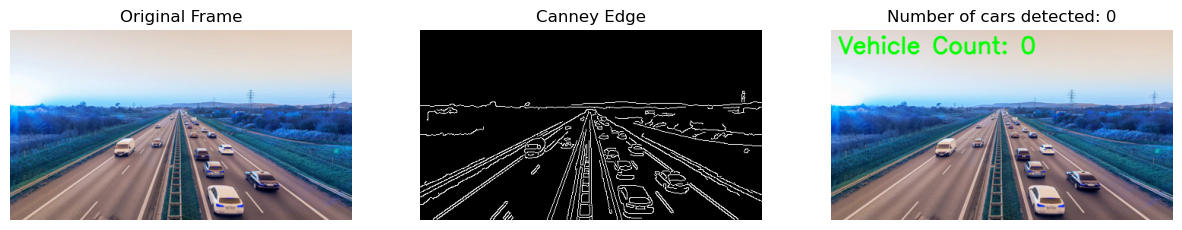
\includegraphics[width=1\linewidth]{edge_detection.png}
    \caption{Canny Edge}
    \label{fig:enter-label}
\end{figure}

\subsection{Background Subtraction}
\begin{itemize}
    \item Gray $\rightarrow$ Gaussian blur (remove noises) $\rightarrow$ Threshold to remove shadows $\rightarrow$ Apply some morphological operations to make sure you have a good mask (getStructuringElement, erode, dilate) $\rightarrow$ Find contour
\end{itemize}
Background subtraction can indeed be limited in its effectiveness for vehicle detection in images. One major challenge arises from the need for a consistent and accurate background model. Background subtraction techniques rely on the assumption that the scene's background remains relatively static over time. However, in real-world scenarios, backgrounds can vary due to changes in lighting conditions, moving objects, or environmental factors.

In the context of vehicle detection from a single picture, background subtraction becomes especially challenging. Unlike in video surveillance applications where a background model can be continuously updated, analyzing a single image lacks the temporal context necessary for accurate background modeling. Without prior knowledge of the background or a reference image captured from the same angle without any vehicles present (often referred to as an empty road picture), background subtraction may yield inaccurate results.
\begin{figure}[H]
    \centering
    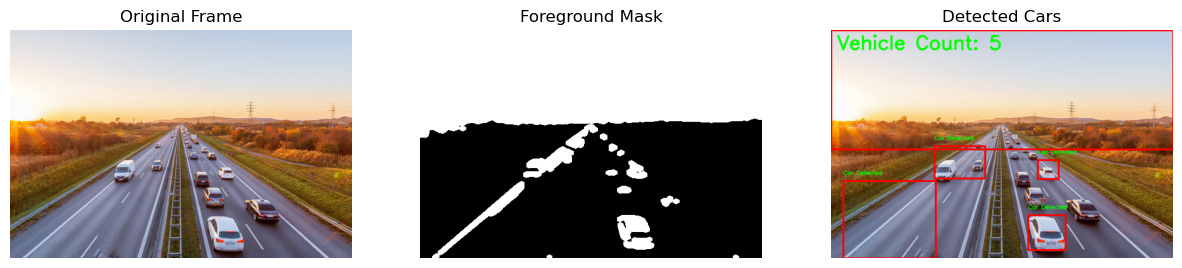
\includegraphics[width=1\linewidth]{background_subtraction.png}
    \caption{Background Subtraction}
    \label{fig:enter-label}
\end{figure}
Background subtraction and edge detection are fundamental techniques used for vehicle detection in images, each with its own set of challenges and limitations. Vehicle detection using edge detection performs poorly due to the complexity of vehicle shapes, ambiguity in edge formation, and inadequate contour formation. Similarly, background subtraction technique is significantly limited when applied to single images due to the need for a consistent and accurate background model. Without an updated background model or a reference image without vehicles, background subtraction often yields inaccurate results. In contrast, cv2.createBackgroundSubtractorMOG(), a Gaussian Mixture-based Background/Foreground Segmentation Algorithm in CV2, performs well with video data by continuously updating the background model.

\subsection{Detection using ML}
To find a better vehicle detector, we tried machine learning-based methods like You-Only-Look-Once (YOLO). YOLO is a popular object detection algorithm known for its speed and accuracy. The architecture of YOLO involves dividing the input image into a grid and predicting bounding boxes and class probabilities for each grid cell simultaneously. This allows YOLO to detect multiple objects in an image in real-time.

Initially, we chose to use YOLOv3. The YOLOv3 object detection model runs a deep learning convolutional neural network (CNN) on an input image to produce network predictions from multiple feature maps. Then, the object detector gathers and decodes predictions to generate the bounding boxes. From these bounding boxes, YOLOv3 uses anchor boxes, where the model predicts these three attributes for each anchor box:
\begin{itemize}
    \item Intersection over union (IoU) — Predicts the objectness score of each anchor box.
    \item Anchor box offsets — Refine the anchor box position.
    \item Class probability — Predicts the class label assigned to each anchor box.
\end{itemize}

We compared the performance of YOLOv3 to other YOLO models, such as YOLOv2 and YOLOv4. From version two to four, improvements to object detection were made in both speed and accuracy through various machine learning techniques and changes in architecture. Since these are pretrained models, we combined all the images into one directory and tested on that.

\section{Experimental Results}
\begin{table}[H]
    \centering
    \begin{tabular}{|m{2.5cm}|m{4.5cm}|m{2.5cm}|m{2.5cm}|m{2.5cm}|}
    \hline
    \textbf{Ground Truth or YOLO model} & \textbf{Detection} & \textbf{Label Instances} & \textbf{Accuracy} & \textbf{Precision, Recall, and F1-Score} \\
    \hline
    \textbf{Ground Truth} & 
    \cellbgimage{image1.png}{\hspace{2.5cm}} & 
    6 cars \newline 0 buses \newline 2 trucks & 
    N/A & N/A \\
    \hline
    \textbf{YOLO v2} & 
    \cellbgimage{image2.png}{\hspace{2.5cm}} & 
    1 car \newline 0 buses \newline 0 trucks & 
    0\% for car \newline 100\% for buses \newline 0\% for trucks & 
    Precision = \newline Recall = \newline F1-Score = \\
    \hline
    \textbf{YOLO v3} & 
    \cellbgimage{image3.png}{\hspace{2.5cm}} & 
    10 cars \newline 0 buses \newline 3 trucks & 
    0\% for car \newline 100\% for buses \newline 0\% for trucks & 
    Precision = \newline Recall = \newline F1-Score = \\
    \hline
    \textbf{YOLO v4} & 
    \cellbgimage{image4.png}{\hspace{2.5cm}} & 
    12 cars \newline 0 buses \newline 3 trucks & 
    0\% for car \newline 100\% for buses \newline 0\% for trucks & 
    Precision = \newline Recall = \newline F1-Score = \\
    \hline
    \end{tabular}
    \caption{Comparison of YOLO Models}
    \label{tab:yolo_comparison}
\end{table}

\begin{table}[H]
    \centering
    \begin{tabular}{|l|c|c|c|}
    \hline
    \textbf{Model} & \textbf{Car Accuracy (\%)} & \textbf{Bus Accuracy (\%)} & \textbf{Truck Accuracy (\%)} \\
    \hline
    YOLOv2 & 18.11 & 78.19 & 2.06 \\
    \hline
    YOLOv3 & 34.57 & 62.55 & 2.06 \\
    \hline
    YOLOv4 & 46.50 & 49.79 & 1.65 \\
    \hline
    \end{tabular}
    \caption{Performance of YOLO Models on the Test Set}
    \label{tab:yolo_performance}
\end{table}


\section{References}
\begin{itemize}
    \item Reference paper on YOLOv3: \url{https://arxiv.org/abs/1804.02767}
    \item YOLOv2, v3, and v4 models: \url{https://github.com/kiyoshiiriemon/yolov4_darknet?tab=readme-ov-file#yolo-v4-v3-and-v2-for-windows-and-linux}
    \item Information about YOLO: \url{https://pjreddie.com/darknet/yolo/}
    \item Dataset: \url{https://universe.roboflow.com/cc-pintel/car-counting}
\end{itemize}

\section{Contributions}


\end{document}
